\chapter[APÊNDICE \ref{Ap:CSD-Exemplos}]{Exemplos de verificação do código de elementos de casca}
\label{Ap:CSD-Exemplos}

% =============================================================================
\section{Problema de \textit{Scordelis-Lo roof}} \label{Ap:SLR}
% =============================================================================

O primeiro exemplo simulado trata-se de um problema comumente encontrado para problemas de cascas, denominado de \textit{Scordelis-Lo roof}, conforme ilustrado na Figura \ref{fig:scordelis}. Esse exemplo se caracteriza por uma cobertura curva sujeita a um carregamento gravitacional $q$, distribuído por unidade de área, na direção $x_3$ para baixo. Os parâmetros geométricos são dados por: comprimento $L=50$, raio de curvatura $R=25$, espessura $t=0,25$ e ângulo $\theta=40^\circ$. O valor da carga aplicada é $q=90$. O material que constitui a cobertura possui módulo de Young $E=4,32\times10^8$ e Poisson nulo. As extremidades estão presas por um diafragma rígido ($u_1=u_3=0$). Os resultados são comparados com os obtidos por \citeonline{BELYTSCHKO1985221,ZHOU2022108568,CHAUDINH2023110222}, os quais apontam que o deslocamento vertical do nó $A$ é de 0,3024.

\begin{figure}[h!]
    \centering
    \caption{Problema de \textit{Scordelis-Lo roof}.}
    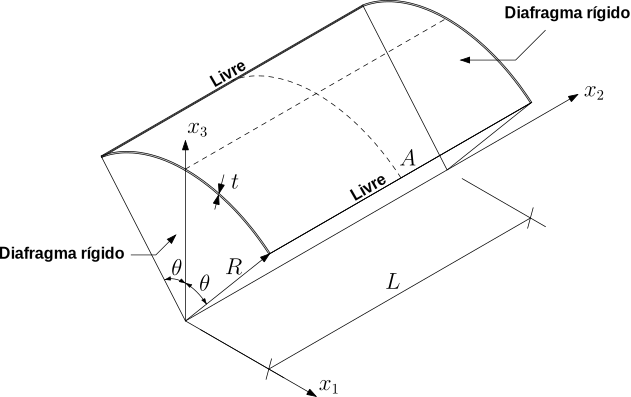
\includegraphics[width=0.75\linewidth]{Figuras/scordelis/scordelis_lo.pdf}
    \\Fonte: Autoria Própria (\the\year).
    \label{fig:scordelis}
\end{figure}

Para a simulação do problema aproveitou-se da simetria da cobertura, o que possibilitou a modelagem de apenas um quarto do problema. Assim utilizou-se uma malha estruturada com orientação à esquerda contendo 512 elementos triangulares de aproximação quadrática, resultando em 7623 graus de liberdade. A malha é apresentada na Figura \ref{fig:scordelis-mesh}. O problema foi considerado em pequenos deslocamentos e deformações, ou seja, utilizou-se somente uma iteração de Newton-Raphson.

\begin{figure}[h!]
    \centering
    \caption{Malha utilizada na simulação de \textit{Scordelis-Lo roof}.}
    \begin{subfigure}{0.35\textwidth}
        \includegraphics[width=\linewidth]{Figuras/scordelis/malha1.png}
        \caption{Perspectiva isométrica.}
    \end{subfigure}
    \begin{subfigure}{0.35\textwidth}
        \includegraphics[width=\linewidth]{Figuras/scordelis/malha2.png}
        \caption{Vista superior.}
    \end{subfigure}
    \\Fonte: Autoria Própria (\the\year).
    \label{fig:scordelis-mesh}
\end{figure}

Dessa forma, chegou-se a um deslocamento de 0,2997 nos cálculos realizados, representando um desvio de 0,8965\% em relação à referência. A Figura \ref{fig:scordelis-displ} apresenta o campo de deslocamentos obtido para um quadrante da cobertura.

\begin{figure}[h!]
    \centering
    \caption{Campos de deslocamentos obtido na simulação de \textit{Scordelis-Lo roof}.}
    \begin{subfigure}{0.05\textwidth}
        \includegraphics[width=\linewidth]{Figuras/scordelis/eixos.png}
    \end{subfigure}
    \begin{subfigure}{0.31\textwidth}
        \includegraphics[width=\linewidth]{Figuras/scordelis/ux.png}
    \end{subfigure}
    \begin{subfigure}{0.31\textwidth}
        \includegraphics[width=\linewidth]{Figuras/scordelis/uy.png}
    \end{subfigure}
    \begin{subfigure}{0.31\textwidth}
        \includegraphics[width=\linewidth]{Figuras/scordelis/uz.png}
    \end{subfigure}
    \\Fonte: Autoria Própria (\the\year).
    \label{fig:scordelis-displ}
\end{figure}

Assim, observa-se que tais campos estão muito semelhantes aos apresentados por \citeonline{ZHOU2022108568}, sendo satisfatoriamente verificada a análise realizada.

Também realizou-se uma análise quanto à convergência da malha, onde dividiu-se as arestas do problema em $N$ partes. A Tabela \ref{tab:scordelis-sol} apresenta os resultados obtidos, sendo os valores do desvio relativo em função do refinamento da malha ilustrados na Figura \ref{fig:shell-static-sol}.

\begin{table}[h!]
    \centering
    \caption{Análise da convergência da malha para o problema de \textit{Scordelis-Lo roof}.}
    \begin{tabular}{ccccc}
        \hline
        $N$ & Número de elementos & Graus de liberdade & Calculado & Desvio relativo \\\hline
        5   & 50                  & 847                & 0,2258    & 25,3287\%       \\
        6   & 72                  & 1183               & 0,2563    & 15,2354\%       \\
        7   & 98                  & 1575               & 0,2736    & 9,5248\%        \\
        8   & 128                 & 2023               & 0,2835    & 6,2563\%        \\
        9   & 162                 & 2527               & 0,2893    & 4,3178\%        \\
        10  & 200                 & 3087               & 0,2930    & 3,1194\%        \\
        11  & 242                 & 3703               & 0,2953    & 2,3479\%        \\
        12  & 288                 & 4375               & 0,2968    & 1,8323\%        \\
        13  & 338                 & 5103               & 0,2979    & 1,4759\%        \\
        14  & 392                 & 5887               & 0,2987    & 1,2219\%        \\
        15  & 450                 & 6727               & 0,2993    & 1,0360\%        \\
        16  & 512                 & 7623               & 0,2997    & 0,8965\%        \\\hline
    \end{tabular}
    \\Fonte:Autoria Própria (\the\year).
    \label{tab:scordelis-sol}
\end{table}

\begin{figure}[h!]
    \centering
    \caption{Desvio relativo do deslocamento vertical do ponto $A$ para diferentes malhas.}
    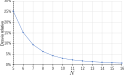
\includegraphics[width=0.75\linewidth]{Figuras/scordelis/static-sol.pdf}
    \\Fonte: Autoria Própria (\the\year).
    \label{fig:shell-static-sol}
\end{figure}

Igualmente analisou-se o resultado com aquele obtido pelo \textit{software} ANSYS, o qual retornou um deslocamento de 0,3020. Assim o desvio relativo do resultado calculado com o do ANSYS é de 0,7616\%. Além disso, observou-se os deslocamentos verticais ao longo da aresta livre da cobertura, os quais são apresentados na Figura \ref{fig:scordelis-graph}.

\begin{figure}[h!]
    \centering
    \caption{Deslocamento vertical ao longo da aresta livre da cobertura.}
    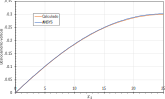
\includegraphics[width=0.7\linewidth]{Figuras/scordelis/deslocamento.pdf}
    \\Fonte: Autoria Própria (\the\year).
    \label{fig:scordelis-graph}
\end{figure}

% =============================================================================
\section{Cilindro biengastado em problema estático} \label{Ap:Shell-cyl}
% =============================================================================

Outro problema comum considera um cilindro sujeito a duas cargas concentradas diametralmente opostas, conforme visto na Figura \ref{fig:cylinder-shell}. As dimensões do problema são: comprimento $L=600$, raio $R=300$ e espessura $t=3$. A carga aplicada é $P=1$. O material que constitui o cilindro possui módulo de elasticidade $E=3\times10^6$ e coeficiente de Poisson $\nu=0,3$. Ambas as extremidades do cilindro estão vinculadas a um diafragma rígido, ou seja, $u_1=u_3=\phi_2=0$. O resultado de referência adotado é de um deslocamento radial de $1,8248\times10^{-5}$ no ponto de aplicação da carga \cite{BELYTSCHKO1985221,CHAUDINH2023110222,ZHOU2022108568}.

\begin{figure}[h!]
    \centering
    \caption{Cilindro submetido a forças concentradas.}
    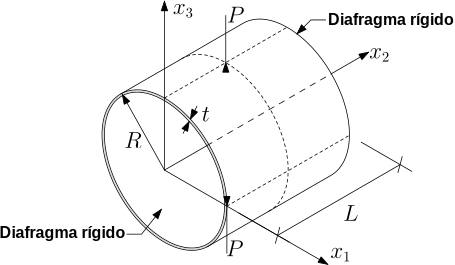
\includegraphics[width=0.65\linewidth]{Figuras/cylinder-shell/cylinder.pdf}
    \\Fonte: Autoria Própria (\the\year).
    \label{fig:cylinder-shell}
\end{figure}

Pelo fato de o problema apresentar simetria, foi estudado somente um octante do problema. Assim utilizou-se uma malha não-estruturada, com refinamento maior próximo ao ponto de aplicação da força, contendo 810 elementos triangulares de aproximação quadrática, contando com um total de 11977 graus de liberdade. A malha utilizada é observada na Figura \ref{fig:cylinder-shell-mesh}. Na simulação adotou-se uma única iteração de Newton-Raphson.

\begin{figure}[h!]
    \centering
    \caption{Malha utilizada na simulação de cilindro biengastado.}
    \includegraphics[width=0.3\linewidth]{Figuras/cylinder-shell/mesh1.png}
    \\Fonte: Autoria Própria (\the\year).
    \label{fig:cylinder-shell-mesh}
\end{figure}

O resultado obtido foi de um deslocamento radial de $1,8135\times10^{-5}$, tendo, portanto, um desvio relativo de $0,6176\%$ em relação à referência. Os campos de deslocamentos obtidos são apresentados na Figura \ref{fig:cylinder-shell-disp}, os quais são muito próximos aos obtidos por \citeonline{ZHOU2022108568}.

\begin{figure}[h!]
    \centering
    \caption{Campos de deslocamentos obtido na simulação de cilindro.}
    \begin{subfigure}{0.075\textwidth}
        \includegraphics[width=\linewidth]{Figuras/cylinder-shell/eixos.png}
    \end{subfigure}
    \begin{subfigure}{0.3\textwidth}
        \includegraphics[width=\linewidth]{Figuras/cylinder-shell/ux.png}
    \end{subfigure}
    \begin{subfigure}{0.3\textwidth}
        \includegraphics[width=\linewidth]{Figuras/cylinder-shell/uy.png}
    \end{subfigure}
    \begin{subfigure}{0.3\textwidth}
        \includegraphics[width=\linewidth]{Figuras/cylinder-shell/uz.png}
    \end{subfigure}
    \\Fonte: Autoria Própria (\the\year).
    \label{fig:cylinder-shell-disp}
\end{figure}

Também se comparou o resultado obtido com relação à uma simulação feita no \textit{software} ANSYS, a qual resultou em um deslocamento de $1,8190\times10^{-5}$. Logo o desvio do resultado calculado com o apresentado pelo ANSYS foi de $0,3007\%$. Além disso, verificou-se o deslocamento radial ao longo das arestas compreendidas pela interseção do cilindro com o plano $x_1=0$ e com $x_2=L/2$. A Figura \ref{fig:cylinder-shell-deslradial} ilustra graficamente os resultados obtidos.

\begin{figure}[h!]
    \centering
    \caption{Deslocamentos radiais ao longo da aresta compreendida pela interseção do cilindro como o plano:}
    \begin{subfigure}{0.49\textwidth}
        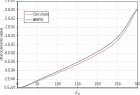
\includegraphics[width=\linewidth]{Figuras/cylinder-shell/deslocamento1.pdf}
        \caption{$x_1=0$}
    \end{subfigure}
    \begin{subfigure}{0.49\textwidth}
        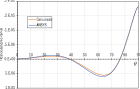
\includegraphics[width=\linewidth]{Figuras/cylinder-shell/deslocamento2.pdf}
        \caption{$x_2=L/2$}
    \end{subfigure}
    \\Fonte: Autoria Própria (\the\year).
    \label{fig:cylinder-shell-deslradial}
\end{figure}

% =============================================================================
\section{Viga engastada em problema dinâmico} \label{Ap:DinBeam}
% =============================================================================

Para verificação do código implementado em problemas dinâmicos, estudou-se  primeiramente o comportamento de uma viga engastada em uma de suas extremidades e sujeita a uma carga $P$ aplicada na extremidade oposta, conforme ilustrado na Figura \ref{fig:viga1}. As dimensões da viga são: comprimento $L=60$ dm, altura $h=3$ dm e largura $b=1$ dm. A força aplicada possui intensidade $P=1,25\times10^{-4}$ Mg$\cdot$dm/(ms)² $H(t)$, sendo $H(t)$ a função de Heavside. O material que compõe a viga possui módulo de Young $E=20$ Mg/[dm$\cdot$(ms)²], coeficiente de Poisson nulo e massa específica $\rho=7\times10^{-3}$ Mg/dm³. O intervalo de tempo analisado foi $t\in[0;675]$ ms discretizado em passos de tempo $\Delta t=0,3377$. A malha de elementos finitos utilizada conta com 32 elementos triangulares de aproximação quadrática, com um total de 693 graus de liberdade, a qual pode ser observada na Figura \ref{fig:viga1-mesh}.

\begin{figure}[h!]
    \centering
    \caption{Desenho esquemático da viga simulada.}
    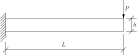
\includegraphics[width=0.5\linewidth]{Figuras/vigas/viga1.pdf}
    \\Fonte: Autoria Própria (\the\year).
    \label{fig:viga1}
\end{figure}

\begin{figure}[h!]
    \centering
    \caption{Malha utilizada na simulação da viga.}
    \includegraphics[width=\linewidth]{Figuras/vigas/mesh1.png}
    \\Fonte: Autoria Própria (\the\year).
    \label{fig:viga1-mesh}
\end{figure}

A modelagem realizada considerou a altura $H$ como a espessura do elemento de casca, sendo a força atuante nessa mesma direção. Assim, observou-se o deslocamento vertical no ponto de aplicação da força. Os resultados obtidos foram comparados com aqueles alcançados a partir de uma modelagem no \textit{software} ANSYS utilizando elementos sólidos 183. a Figura \ref{fig:res-viga1} apresenta os resultados calculados.

\begin{figure}[h!]
    \centering
    \caption{Deslocamento vertical no ponto de aplicação da força ao longo do tempo.}
    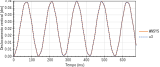
\includegraphics[width=\linewidth]{Figuras/vigas/res1.pdf}
    \\Fonte: Autoria Própria (\the\year).
    \label{fig:res-viga1}
\end{figure}

Observa-se nesse caso uma boa concordância entre os resultados apresentados pelo ANSYS e os obtidos pelo código desenvolvido, sendo verificada a eficácia nesse exemplo.

Outro exemplo trata-se de uma viga biengastada com uma carga aplicada em seu centro, conforme mostrado na Figura \ref{fig:viga2}. Nesse exemplo considerou-se um comprimento $L=20$ in, com seção transversal de $b\times h=1,0\times0,125$ in². O material que constitui a viga possui módulo de Young $E=3\times10^{7}$ lb/in², coeficiente de Poisson nulo e massa específica de $\rho=2,6\times10^{-4}$ lb$\cdot$s²/in$^4$. A força aplicada foi de $P=640$ lb constante durante todo o período de análise, de $t\in[0;5]$ ms, o qual foi discretizado em passos de tempo de $\Delta t=25\ \mu$ s. A malha de elementos finitos (Figura \ref{fig:viga2-mesh}) possui 132 elementos triangulares de aproximação quadrática, totalizando 2331 graus de liberdade. A espessura do elemento de casca foi considerada como a direção da altura $H$ da viga.

\begin{figure}[h!]
    \centering
    \caption{Desenho esquemático da viga biengastada simulada.}
    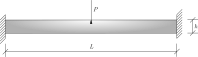
\includegraphics[width=0.6\linewidth]{Figuras/vigas/viga2.pdf}
    \\Fonte: Autoria Própria (\the\year).
    \label{fig:viga2}
\end{figure}

\begin{figure}[h!]
    \centering
    \caption{Malha utilizada na simulação da viga biengastada.}
    \includegraphics[width=\linewidth]{Figuras/vigas/mesh2.png}
    \\Fonte: Autoria Própria (\the\year).
    \label{fig:viga2-mesh}
\end{figure}

Os resultados calculados foram comparados com os apresentados pelo ANSYS, a partir do elemento 183, e por \cite{mondkar1977ansa}. A Figura \ref{fig:res-viga2} exibe os resultados obtidos.

\begin{figure}[h!]
    \centering
    \caption{Deslocamento vertical no centro da viga biengastada ao longo do tempo.}
    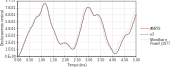
\includegraphics[width=\linewidth]{Figuras/vigas/res2.pdf}
    \\Fonte: Autoria Própria (\the\year).
    \label{fig:res-viga2}
\end{figure}

Verifica-se uma boa concordância entre os resultados obtidos pela análise por ambos os valores de referência, sendo assim, averiguada a eficácia do código nesse exemplo.